\section{两个对数的乘积}\label{sec:14}

在本节中, 我们将我们的方法应用到某些对数的乘积上. 
Baker 定理 \cite{Bak64} 给出了关于对数线性形式的决定性结果（甚至是在 \(\overline{\mathbf{Q}}\) 上）, 
但我们仍然不知道如何证明 \(\log 2 \cdot \log 3\) 以及 \(\pi \cdot \log 2\) 是无理数. 
虽然我们的方法（目前！）同样无法处理那些情况, 但我们确实证明了定理 C, 我们在此再次予以回顾：

\begin{theorem}\label{thm:14.0.1}
设 \(m, n \in \mathbf{Z} \setminus \{-1, 0\}\) 是满足 \(\left| \frac{m}{n} - 1 \right| < \frac{1}{10^6}\) 的有理整数. 
那么
\begin{equation}\label{eq:14.0.2}
\log\left(1 + \frac{1}{m}\right)\log\left(1 + \frac{1}{n}\right)
\end{equation}
是无理数. 
此外, 当 \(m \neq n\) 时, 以下四个数在 \(\mathbf{Q}\) 上是线性无关的:
\begin{equation}\label{eq:14.0.3}
1, \quad \log\left(1+\frac{1}{m}\right), \quad \log\left(1+\frac{1}{n}\right), \quad \log\left(1+\frac{1}{m}\right)\log\left(1+\frac{1}{n}\right).
\end{equation}
\end{theorem}

\begin{remark}\label{rem:14.0.4}
我们当然可以通过我们的方法改进常数 \(10^{-6}\), 
但一些计算表明, 人们不太可能做得到比（比如） \(10^{-4}\) 更好的结果, 
以及可能根本无法达到那么远；我们选择这个常数是为了其相对简单性. \end{remark}

\(m=n\) 的退化情况是 \(\mathbf{Q} \setminus \{1\}\) 中有理数 r 的 \(\log r\) 超越性的平凡推论, 
因此我们将假设 \(m \neq n\). 
我们首先召回关于
\begin{equation}\label{eq:14.0.5}
\log\left(1 + \frac{1}{m}\right)
\end{equation}
对于 \(m \geq 1\) 的无理性的一个证明（源于 \cite{AR80}\cite{Chu79}\cite{vdP79}）, 该证明基于 Ap{\'e}ry 极限方法. 
这与我们在基本注记 2.10.1 中叙述的构造以及在第 3.3.7 节中关于对数函数的 Hermite--Pad{\'e} 构造是密切相关的.

设 a > 1 是一个有理整数. 函数
\begin{equation}\label{eq:14.0.6}
A(a,x) := \frac{1}{\sqrt{1 - 2ax + x^2}} = \sum_{n=0}^{\infty} u_n(a)x^n
\end{equation}
当 a 是奇数时属于 \(\mathbf{Z}[x]\), 否则属于 \(\mathbf{Z}[x/2]\), 
并且满足一阶线性 ODE:
\begin{equation}\label{eq:14.0.7}
(1 - 2ax + x^2)y' + (x - a)y = 0.
\end{equation}
存在唯一的有理系数全纯非齐次 ODE
\[ (1 - 2ax + x^2)y' + (x - a)y = 1 \]
的在 0 处消逝的全纯解；它由下式给出:
\begin{equation}\label{eq:14.0.8}
H(a,x) := \frac{1}{\sqrt{1 - 2ax + x^2}} \int_0^x \frac{dt}{\sqrt{1 - 2at + t^2}}
\end{equation}
\[ = \frac{1}{\sqrt{1 - 2ax + x^2}} \left( \log\left(a - x - \sqrt{1 - 2ax + x^2}\right) - \log(a - 1) \right) \]
\[ = x + \frac{ax^2}{2} + \frac{(3a^2 - 1)x^3}{6} + \dots = \sum_{n=0}^{\infty} v_n(a)x^n \in \mathbf{Q}[x], \]
并且此外, 它的系数 \(v_n(a)\) 当 a 是奇数时满足 \([1, 2, \ldots, n]v_n(a) \in \mathbf{Z}\), 
否则满足 \([1, 2, \ldots, n]2^n v_n(a) \in \mathbf{Z}\). 
根据 \eqref{eq:14.0.8}, 我们有公式:
\[ H(a,x) - \frac{1}{2}\log\left(\frac{a+1}{a-1}\right)A(a,x) = \frac{1}{\sqrt{1-2ax+x^2}} \int_{a-\sqrt{a^2-1}}^{x} \frac{dt}{\sqrt{1-2at+t^2}} \]
其右手边由于在沿着包围该奇点 \(x=a-\sqrt{a^2-1}\) 
的简单回路进行解析延拓后两个因子的相乘 \((-1)\) 单值性而在该奇点处超收敛. 
这与第 2.11.12 节中关于超收敛的机制以及在第 11.1 节中关于 Eisenstein 级数 A 以及 Eichler 积分 \(B-\frac{1}{2}L(2,\chi_{-3})\) 的消去模形式权重的机制是完全相同的. 
当前研究的情况很容易被看出：在不改变记号的前提下, 
等价于由对数函数的对角 Hermite--Pad{\'e} 逼近表产生的一阶线性 ODE \eqref{eq:3.3.12} 以及公式 \eqref{eq:3.3.8}, 
这我们在第 3.3.7 以及 3.3.13 节中已经叙述过.

紧接着有:
\begin{equation}\label{eq:14.0.9}
\lim_{n \to \infty} \frac{v_n(a)}{u_n(a)} \to \frac{1}{2} \log \left( \frac{a+1}{a-1} \right)
\end{equation}
收敛得足够快, 以便在不等式:
\[ 5.828... = 3 + 2\sqrt{2} > e = 2.718..., \]
\[ 7.872... = 4 + \sqrt{15} > 2 \cdot e = 5.43656... \]
的前提下证明对于任意奇数 \(a \geq 3\) 以及任意偶数 \(a \geq 4\) 这一数量的无理性. 
如果设 a = 1 + 2m, 那么有
\[ \log\left(\frac{a+1}{a-1}\right) = \log\left(1 + \frac{1}{m}\right), \]
并随之如所期望的那样给出了数量 \eqref{eq:14.0.5} 的无理性（其通过对该论证 of 较好研究, 被 Chudnovsky \cite{Chu79}\cite{Chu83b} 进一步精细化为了相当卓越的无理数测度）.

我们现在考虑数量:
\begin{equation}\label{eq:14.0.10}
\log\left(\frac{a+1}{a-1}\right)\log\left(\frac{b+1}{b-1}\right)
\end{equation}
对于一对不同的有理整数 \(a \neq b\) 的算术性质. 
由 \eqref{eq:14.0.9} 显然有:
\begin{equation}\label{eq:14.0.11}
\lim_{n \to \infty} \frac{v_n(a)}{u_n(a)} \cdot \frac{v_n(b)}{u_n(b)} \to \frac{1}{4} \log\left(\frac{a+1}{a-1}\right) \log\left(\frac{b+1}{b-1}\right).
\end{equation}
然而, 这一收敛显然无法通过任何初等分析快到足以证明右手边的无理性. 
我们仍然将会看到：只要 a/b 足够接近 1, 
这一数量就可以通过我们基于底层生成级数的函数论性质以及 Hadamard 乘积运算（它允许构造具有所需 Ap{\'e}ry 极限的新 G-函数）的基本性质的全新方法来接近.

对于每一对整数 a, b \(\in \mathbf{Z} \setminus \{-1, 0, 1\}\), 让我们写出:
\[ \eta_a := \frac{1}{2} \log \left( \frac{a+1}{a-1} \right), \quad \eta_b := \frac{1}{2} \log \left( \frac{b+1}{b-1} \right), \]
\[ \eta_{a,b} := \eta_a \eta_b := \frac{1}{4} \log \left( \frac{a+1}{a-1} \right) \log \left( \frac{b+1}{b-1} \right). \]
我们将假设 \(a \neq \pm b\), 因为 \(\eta_{a,a} = -\eta_{a,-a} = \eta_a^2\) 的无理性以及超越性已经是已知的. 
我们对于周期乘积 \(\eta_{a,b} = \eta_a \eta_b\) 算术性质的研究途径是通过底层 G-函数的 Hadamard 乘积进行的.

\subsection{Hadamard 乘积以及 Ap{\'e}ry 极限}\label{sec:14.1}

设 \(\star\) 表示在幂级数上的 Hadamard 乘积运算：\((\sum a_n x^n) \star (\sum b_n x^n) := \sum a_n b_n x^n\). 
函数
\begin{equation}\label{eq:14.1.1}
P_A(x) := A(a, x) \star A(b, x) = \sum u_n(a)u_n(b)x^n
\end{equation}
满足以下形式的一阶线性 ODE \(\mathcal{M}(P_A(x)) = 0\):
\begin{equation}\label{eq:14.1.2}
(-1+x)x(1+x)(1-4abx-2x^2+4a^2x^2+4b^2x^2-4abx^3+x^4)y''
\end{equation}
\[ +(-1+8abx+5x^2-12a^2x^2-12b^2x^2+16abx^3-7x^4+4a^2x^4+4b^2x^4-8abx^5+3x^6)y' \]
\[ +(ab-(-1+3a^2+3b^2)x+8abx^2-(2+a^2+b^2)x^3-abx^4+x^5)y=0. \]
点 x = 1 以及 x = -1 是该 ODE 的表观奇异点, 
只要分别满足 \(a-b \neq 0\) 以及 \(a+b \neq 0\). 
这既根据 Hadamard 乘积的一般性质 \cite{Her1893} 成立, 
也可以直接通过计算指标方程（为 \(R(R-2)=0\)）以及确立存在两个线性无关的幂级数解来予以验证. 
例如, 对于推定解 \(\sum c_n(x+1)^n\), 系数满足如下递推关系:
\[ (a+b)^2 n(n-2)c_n = 12(a+b)^2 c_{n-1} - 4(a+b)^2 (n-2) c_{n-1} (7n-9)(n-2) + 6(a+b)^2 c_{n-2} + (n-2) c_{n-2}(\ldots) + \dots, \]
这蕴含了存在至少一个具有形式 \(x^2 + \dots\) 的解, 
但还存在另一个具有如下形式的解:
\[ 1 + \frac{(x+1)}{2} - \frac{(x+1)^3}{4} + \dots \in \mathbf{Q}[a, b, x+1]. \]
对于 x = 1 的情况也是完全类似的. 
四阶多项式的四个根恰好是各一阶 ODE 奇异点的乘积, 
即:
\[ \left(a\pm\sqrt{a^2-1}\right) \left(b\pm\sqrt{b^2-1}\right). \]

\begin{remark}[Basic Remark 14.1.3]\label{rem:14.1.3}
如果 a 以及 b 很大且 a/b 以及接近 1, 
那么 \eqref{eq:14.1.2} 的四个非零有限奇异点分组如下:
\begin{itemize}
  \item[(1)] 一个奇异点 \(\alpha\) 以及接近 0.
  \item[(2)] 两个奇异点以及接近 1.
  \item[(3)] 一个以及巨大的奇异点（“接近 \(\infty\)”）.
\end{itemize}
除了这些之外, 0 以及 \(\infty\) 自身也是（本质）奇异点. 
我们将在假设量 \eqref{eq:14.0.3} 在 \(\mathbf{Q}\) 上线性相关的条件下, 
构造一个具有分母类型 \(\tau = [1,2,\dots,n]^2\) 
且满足 \eqref{eq:14.1.2} 的非齐次版本、并在 \(\alpha\) 之外超收敛的有理系数函数 \(H(x)\). 
当在 \(\mathbf{P}^1 \setminus \{0,1,\infty\}\) 上研究具有分母类型 \(\tau = [1,2,\dots,n]^2\) 
的函数时, 根据第 2.9.5 节, 我们被要求选择一个满足 \(\varphi(0)=0\) 以及 \(\varphi^{-1}(0)=\{0\}\) 
的辅助全纯映射 \(\varphi: \mathbf{D} \to \mathbf{C} \setminus \{1\}\). 
如果我们限制 \(\varphi\) 到对于任意 \(\epsilon \in (0,1/2]\) 的圆盘 \(D(0,1-\epsilon)\) 上, 
那么 \(\varphi\) 的值域将避开包含 1 的一个微小开球以及包含 \(\infty\) 的一个开球, 
并满足 \(\#\varphi^{-1}(\alpha)=1\). 
这正是我们的 holonomy 边界可以被应用的设定, 
因为我们不仅可以纳入形式函数 \(H(x)\) 以及它们的导数, 
还可以纳入我们在第 10 节中设计的、在 \(\mathbf{P}^1 \setminus \{0,1,\infty\}\) 上的纯函数. 
在实际中, 我们的映射 \(\varphi\) 具有 \(\lambda \circ \psi\) 的形式, 
或者在等价的 \(\mathbf{P}^1 \setminus \{0,4,\infty\}\) 设定下, 具有 \(h \circ \psi\) 的形式, 
其中 \(\psi : \overline{\mathbf{D}} \to \mathbf{D}\) 
是我们在 \(\mathbf{D}\) 内一合适选择区域的 Riemann 映射. 
但是, 尽管函数 \(\lambda\) 排除了在 \(\mathbf{D}\) 上的 1, 
但为了排除与 1 相差 \(\epsilon\) 以内的值, 
就需要 \(\psi\) 具有明显更小的共形半径, 
除非 \(\epsilon\) 是以及微小的. 
例如, 如果 \(\psi(\mathbf{D})\) 在 \(\mathbf{D}\) 内的像包含了点 3/4, 
那么在 \(\mathbf{D}\) 上的 \(\varphi = \lambda \circ \psi\) 
将已经包含了值:
\[ \lambda(3/4) = 0.9999999999999999332\dots \]
这一数值特征是最终迫使我们要假设 \(|m/n-1|\) 是以及微小的值的原因. \end{remark}

\subsubsection{超收敛空间}\label{sec:14.1.4}

我们现在考虑对乘积 ODE \eqref{eq:14.1.2} 的非齐次形式的解. 
用 \(\mathcal{M}\) 表示 \eqref{eq:14.1.2} 的对应微分算子, 
那么我们也有以下恒等式:
\[ \mathcal{M}(H(a,x) \star A(b,x)) = -b + 3ax - 3bx^{2} + ax^{3}, \]
\[ \mathcal{M}(A(a,x) \star H(b,x)) = -a + 3bx - 3ax^{2} + bx^{3}, \]
\[ \mathcal{M}(H(a,x) \star H(b,x)) = -1 + 2x^{2} - x^{4}. \]
我们进一步声称, 函数:
\begin{equation}\label{eq:14.1.5}
P_{a} := (H(a,x) - \eta_{a}A(a,x)) \star A(b,x) = \sum (v_{n}(a) - \eta_{a}u_{n}(a))u_{n}(b)x^{n},
\end{equation}
\[ P_{b} := A(a,x) \star (H(b,x) - \eta_{b}A(b,x)) = \sum u_{n}(a)(v_{n}(b) - \eta_{b}u_{n}(b))x^{n}, \]
\[ P_{ab} := H(a,x) \star H(b,x) - \eta_{a,b}A(a,x) \star A(b,x) = \sum (v_{n}(a)v_{n}(b) - \eta_{a,b}u_{n}(a)u_{n}(b))x^{n} \]
\[
\begin{aligned}
&= \sum \left( \eta_{a}u_{n}(a)(v_{n}(b) - \eta_{b}u_{n}(b)) + \eta_{b}(v_{n}(a) - \eta_{a}u_{n}(a))u_{n}(b) \right) x^{n} \\
&\quad + \sum (v_{n}(a) - \eta_{a}u_{n}(a))(v_{n}(b) - \eta_{b}u_{n}(b))x^{n}
\end{aligned}
\]
是超越了最小奇异点 \((a - \sqrt{a^2 - 1})(b - \sqrt{b^2 - 1})\) 之外超收敛的. 
这根据以下估计而成立:
\[ |v_n(a) - \eta_a u_n(a)| = O((a - \sqrt{a^2 - 1})^{n(1 - \epsilon)}), \]
\[ |v_n(b) - \eta_b u_n(b)| = O((b - \sqrt{b^2 - 1})^{n(1 - \epsilon)}), \]
伴随着:
\[ |v_n(a)|, |u_n(a)| = O((a + \sqrt{a^2 - 1})^{n(1+\epsilon)}), \]
\[ |v_n(b)|, |u_n(b)| = O((b + \sqrt{b^2 - 1})^{n(1+\epsilon)}). \]

我们可以将 \(P_{ab}\) 在 \eqref{eq:14.1.5} 最后两行中的级数分解写为以下等同形式:
\[
\begin{aligned}
P_{ab} &= \eta_a A(a, x) \star (H(b, x) - \eta_b A(b, x)) + \eta_b (H(a, x) - \eta_a A(a, x)) \star A(b, x) \\
&\quad + (H(a, x) - \eta_a A(a, x)) \star (H(b, x) - \eta_b A(b, x)).
\end{aligned}
\]
我们在此处利用的一般事实 \cite{Her1893} 是：任意一组 holonomic 幂级数的 Hadamard 乘积仍然是超收敛的, 
只要其中至少有一个是第 2.9 节意义下的超收敛分支. 
这在本质上与 Jacobson 恒等式 \(1-xy=(1-x)+(1-y)-(1-x)(1-y)\) 结合在了一起, 
后者例如在有限 p-群的 \(\mathbf{F}_p\)-群环的增广理想的幂零性证明中是熟知的.

\subsubsection{不可能的 G-函数的构造}\label{sec:14.1.6}

假设现在直到定理 14.0.1 证明的末尾, 
都存在不全为零的整数 \(r_0, r_a, r_b\) 以及 \(r_{ab}\), 使得:
\begin{equation}\label{eq:14.1.7}
r_a \eta_a + r_b \eta_b + r_{ab} \eta_{a,b} = r_0.
\end{equation}
那么线性组合
\begin{equation}\label{eq:14.1.8}
P := r_{a}P_{a} + r_{b}P_{b} + r_{ab}P_{ab} = r_{a}H(a, x) \star A(b, x) + r_{b}A(a, x) \star H(b, x) + r_{ab}H(a, x) \star H(b, x) + r_{0}A(a, x) \star A(b, x)
\end{equation}
\[ = \sum c_{n}(a, b)x^{n} \in \mathbf{Q}[\![x]\!] \]
也属于第 14.1.4 节中的超收敛空间, 
但现在它具有有理数系数. 
这就是依赖于我们关于线性相关性 \eqref{eq:14.1.7} 的荒谬假设、而将最终被我们的 holonomy 边界反驳的该 G-函数. 
该不可能函数的解析性质源于第 14.1.4 节中的超收敛性；我们现在收集其算术性质. 
如果 a 以及 b 都是奇数, 那么 \(u_n(a), u_n(b) \in \mathbf{Z}\) 
并且此外 \([1, 2, \ldots, n]v_n(a)\) 以及 \([1, 2, \ldots, n]v_n(b)\) 都在 \(\mathbf{Z}\) 中. 
因此, 在 Hadamard 乘积构造下:
\[ [1, 2, \dots, n]^2 c_n(a, b) \in \mathbf{Z}. \]
此外, 伴随 a=1+2m 以及 b=1+2n, 线性关系 \eqref{eq:14.1.7} 的不存在性恰好是定理 C 的结论. 
（条件 \(a,b\in \mathbf{Z}\setminus \{-1,0,1\}\) 变为了 \(m,n\in \mathbf{Z}\setminus \{-1,0\}\).） 
因此, 为了证明定理 C, 只要假设存在关系 \eqref{eq:14.1.7} 以及如 \eqref{eq:14.1.8} 中的函数 P(x), 
并确立一个矛盾即为足够.

\begin{definition}\label{def:14.1.9}
在 \(r_a, r_b\) 以及 \(r_{ab}\) 满足 \eqref{eq:14.1.7} 的前提下, 
设 P(x) 如等式 \eqref{eq:14.1.8} 中定义, 并且设:
\[ G(y) := P(x) + P\left(\frac{x}{x-1}\right) \in \mathbf{Q}[\![y]\!]. \]
伴随如 \eqref{eq:14.1.1} 的 \(P_A(x) = A(a, x) \star A(b, x)\), 设:
\[ G_A(y) := P_A(x) + P_A\left(\frac{x}{x-1}\right), \]
并因此当 a, b 是奇数时有 \(G_A(y) \in \mathbf{Z}[\![y]\!]\), 否则有 \(G_A(y) \in \mathbf{Z}[\![1/2]\!][\![y]\!]\). \(\vartriangle\)
\end{definition}

与定理 A 的证明以及相似, 我们将在第 9 节的字典中研究 \(Y_0(2)\) 情况, 
以及反驳存在具有分母类型 \([1, \ldots, 2n]^2\) 
以及“接近于”我们在第 10 节中研究的 \(\mathbf{P}^1 \setminus \{0, 4, \infty\}\) 类型的 G-函数 \(G \in \mathbf{Q}[\![y]\!]\). 
我们在下文命题 14.1.11 中记录 G 的这些性质, 在此之前首先给出以下定义:

\begin{definition}\label{def:14.1.10}
令 \(y_{a^{\pm},b^{\pm}}\) 表示由下式给出的 \(y:=\pi(x)=x+\frac{x}{x-1}\) 的像:
\[ x = \left(a \pm \sqrt{a^2 - 1}\right) \left(b \pm \sqrt{b^2 - 1}\right), \]
其中考虑了所有四个符号对. 用 \(\mathcal{L}\) 表示 \(\mathcal{M}\) 在 \(\pi\) 下的推前, 
从而满足 \(\mathcal{L}(G_A(y)) = 0\). \(\vartriangle\)
\end{definition}

我们当前的讨论是有条件地建立在假设 \(\mathbf{Z}\)-线性关系 \eqref{eq:14.1.7} 成立的前提下的. 
在此处, 我们做出额外的假设：有理整数 \(a, b \in \mathbf{Z} \setminus \{\pm 1\}\) 是奇数.

\begin{proposition}\label{prop:14.1.11}
对于奇数 \(a, b \in \mathbf{Z} \setminus \{\pm 1\}\), 
第 14.1.9 节中定义的函数 \(G(y) \in \mathbf{Q}[\![y]\!]\) 以及 \(G_A(y) \in \mathbf{Q}[\![y]\!]\) 
分别具有分母类型 \([1, \ldots, 2n]^2\) 以及 1. 
此外, \(\mathcal{L}(G_A(y)) = 0\) 并且对于 \(\mathbf{Q}(y)\) 上的某个非零线性微分算子 \(\mathcal{L}\) 
有 \(\mathcal{L}(G(y)) \in \mathbf{Q}[\![y]\!]\), 该算子满足:
\begin{itemize}
  \item[(1)] \(\mathcal{L}\) 除了 \(y \in \{0, 4, y_{a^{\pm}, b^{\pm}}, \infty\}\) 之外没有别的奇异点.
  \item[(2)] \(\mathcal{L}\) 绕奇异点 y=4 具有 \(\mathbb{Z}/2\) 局部单值性.
\end{itemize}
\end{proposition}

我们将在下文第 14.2 节中显式地写出 \(\mathcal{L}\)； 
多项式 \(\mathcal{L}(G(y)) \in \mathbf{Q}[a, b, y]\) 的确切形式可以被计算出来, 但这并不重要.

\subsection{微分方程 \(\mathcal{L}(G_A) = 0\)}\label{sec:14.2}

在给出引理 14.3.1（引理 12.1.1 的对应物）的表述以及证明之前, 
我们应该更详细地检验 ODE \(\mathcal{L}(G_A) = 0\). 
由于该计算的长度, 与在证明引理 12.1.1 期间证明有关 Zagier 函数的相关事实相比, 
将该计算单独陈述、而不是与引理 14.3.1 的证明交织在一起是更有道理的. 
然而, 读者可能以及希望提前看看引理 14.3.1 的表述, 
以了解我们要往何处去. 
我们从 \eqref{eq:14.1.2} 计算出 \(\mathcal{L}\) 的以下显式形式:
\[ \mathcal{L}(G_A) = \sum_{i=0}^{4} c_i(y) G_A^{(i)}(y) = 0, \]
其中 \(c_i(y)\) 是满足下式的某些多项式:
\begin{equation}\label{eq:14.2.1}
c_{0}(y) = R_{12}(y), \qquad c_{1}(y) = R_{16,A}(y), \qquad c_{2}(y) = yR_{16,B}(y),
\end{equation}
\[ c_{3}(y) = y^{2}(y - 4)R_{15}(y), \qquad c_{4}(y) = (y - 4)^{2}y^{3}R_{4}(y)R_{10}(y). \]
在此, \(R_d(y)\) 表示 \(\mathbf{Q}(a, b, y)\) 中关于 y 的次数为 d 的不可约多项式, 
并且下标 A 以及 B 表示 \(R_{16,A}\) 以及 \(R_{16,B}\) 是不同的. 
多项式
\[ (1-x)^4 R_4 \left(x + \frac{x}{x-1}\right) \]
具有 \((a\pm \sqrt{a^2 - 1})(b\pm \sqrt{b^2 - 1})\) 作为其 8 个根之中的 4 个, 
以及这些根在对合自同构 \(w(x) = x/(x-1)\) 下的像. 
特别地, \(R_4(y)\) 的根是 \(\mathcal{L}\) 的奇异点 \(y_{a^{\pm},b^{\pm}}\). 
多项式 \(R_4(y)\) 以及由下式显式地给出:
\[ R_4(y) = 1 + 4y - 8a^2y - 4aby - 8b^2y + 16a^2b^2y + 4y^2 - 12a^2y^2 + 16a^4y^2 \]
\[ + 20aby^2 - 16a^3by^2 - 12b^2y^2 - 16ab^3y^2 + 16b^4y^2 - 8a^2y^3 + 16aby^3 \]
\[ - 16a^3by^3 - 8b^2y^3 + 32a^2b^2y^3 - 16ab^3y^3 + 4a^2y^4 - 8aby^4 + 4b^2y^4. \]
与 \(R_4(y)\) 以及在 \eqref{eq:14.2.1} 的 \(c_4(y)\) 中出现的 y 以及 \((y-4)\) 
的伴随方幂不同, \(R_{10}(y)\) 的根并不是 \(\mathcal{L}\) 的真实奇异点. 
更确切地, 只要 \(R_{10}(y)\) 的根与 \(R_4(y)y(y-4)\) 的根是两两不同的, 这一结论就是成立的, 
且在我们的假设下, 这根据下文证明的引理 14.2.6 以及 14.2.4 是满足的. 
多项式 \(R_{10}(y)\) 也可被显式地计算出来:
\[ R_{10}(y) = 4a^2b^2 + 9y - 27a^2y - 102aby + 144a^3by - 27b^2y + 207a^2b^2y - 128a^4b^2y \]
\[ + 144ab^3y - 160a^3b^3y - 128a^2b^4y + 64y^2 - 93a^2y^2 + 228a^4y^2 - 284aby^2 + 740a^3by^2 \]
\[ - 992a^5by^2 - 93b^2y^2 - 818a^2b^2y^2 - 16a^4b^2y^2 + 740ab^3y^2 + 1208a^3b^3y^2 + 228b^4y^2 - 16a^2b^4y^2 \]
\[ + 64a^4b^4y^2 - 992ab^5y^2 + 164y^3 - 132a^2y^3 - 804a^4y^3 + 432a^6y^3 - 100aby^3 + 1218a^3by^3 \]
\[ + 2360a^5by^3 - 1536a^7by^3 - 132b^2y^3 - 1108a^2b^2y^3 - 856a^4b^2y^3 + 1856a^6b^2y^3 + 1218ab^3y^3 \]
\[ - 3120a^3b^3y^3 - 448a^5b^3y^3 - 804b^4y^3 - 856a^2b^4y^3 - 16a^4b^4y^3 + 2360ab^5y^3 - 448a^3b^5y^3 + 432b^6y^3 \]
\[ + 1856a^2b^6y^3 - 1536ab^7y^3 + 168y^4 - 18a^2y^4 - 1476a^4y^4 + 432a^6y^4 - 108aby^4 - 840a^3by^4 \]
\[ + 688a^5by^4 + 384a^7by^4 - 18b^2y^4 + 4384a^2b^2y^4 - 8864a^4b^2y^4 + 4384a^6b^2y^4 - 840ab^3y^4 \]
\[ + 15744a^3b^3y^4 - 11744a^5b^3y^4 - 1476b^4y^4 - 8864a^2b^4y^4 + 13920a^4b^4y^4 + 688ab^5y^4 - 11744a^3b^5y^4 \]
\[ + 432b^6y^4 + 4384a^2b^6y^4 + 384ab^7y^4 + 32y^5 + 180a^2y^5 + 2467a^4y^5 + 792a^6y^5 - 720a^8y^5 \]
\[ - 424aby^5 - 4228a^3by^5 + 440a^5by^5 + 1824a^7by^5 + 180b^2y^5 + 3554a^2b^2y^5 \]
\[ - 15928a^4b^2y^5 + 5104a^6b^2y^5 - 4228ab^3y^5 + 29392a^3b^3y^5 - 25088a^5b^3y^5 + 2467b^4y^5 \]
\[ - 440ab^5y^5 - 25088a^3b^5y^5 + 792b^6y^5 + 5104a^2b^6y^5 + 1824ab^7y^5 - 720b^8y^5 - 32y^6 - 336a^2y^6 \]
\[ + 258a^4y^6 - 3840a^6y^6 + 480a^8y^6 + 736aby^6 + 1064a^3by^6 + 6680a^5by^6 - 4320a^7by^6 - 336b^2y^6 \]
\[ - 2676a^2b^2y^6 + 6976a^4b^2y^6 + 10688a^6b^2y^6 + 1064ab^3y^6 - 19632a^3b^3y^6 - 12256a^5b^3y^6 \]
\[ + 258b^4y^6 + 6976a^2b^4y^6 + 10816a^4b^4y^6 + 6680ab^5y^6 - 12256a^3b^5y^6 - 3840b^6y^6 \]
\[ + 10688a^2b^6y^6 - 4320ab^7y^6 + 480b^8y^6 - 576a^2y^7 - 1392a^4y^7 + 4368a^6y^7 + 1152aby^7 \]
\[ + 5312a^3by^7 - 12848a^5by^7 + 576ab^7y^7 - 576b^2y^7 - 7840a^2b^2y^7 + 12912a^4b^2y^7 - 1104a^6b^2y^7 \]
\[ + 5312a^3by^7 - 8864a^3b^3y^7 - 768a^5b^3y^7 - 1392b^4y^7 + 12912a^2b^4y^7 + 2592a^4b^4y^7 - 12848ab^5y^7 \]
\[ - 768a^3b^5y^7 + 4368b^6y^7 - 1104a^2b^6y^7 + 576ab^7y^7 + 192a^2y^8 + 168a^4y^8 - 960a^6y^8 \]
\[ - 384aby^8 - 864a^3by^8 + 1568a^5by^8 + 192b^2y^8 + 1392a^2b^2y^8 + 2368a^4b^2y^8 - 288a^6b^2y^8 \]
\[ - 864ab^3y^8 - 5952a^3b^3y^8 + 1152a^5b^3y^8 + 168b^4y^8 + 2368a^2b^4y^8 - 1728a^4b^4y^8 + 1568ab^5y^8 \]
\[ + 1152a^3b^5y^8 - 960b^6y^8 - 288a^2b^6y^8 + 160a^4y^9 - 640a^3by^9 + 448a^5by^9 + 960a^2b^2y^9 \]
\[ - 1792a^4b^2y^9 - 640ab^3y^9 + 2688a^3b^3y^9 + 160b^4y^9 - 1792a^2b^4y^9 + 448ab^5y^9 - 32a^4y^{10} \]
\[ + 128a^3by^{10} - 192a^2b^2y^{10} + 128ab^3y^{10} - 32b^4y^{10}. \]

我们还发现
\[ \frac{c_3(y)}{c_4(y)} = \frac{d}{dy} \log \left( \frac{(y-4)^3 y^5 R_4(y)^3}{R_{10}(y)} \right). \]
我们计算出 \(R_{10}(y)\) 的判别式具有以下形式（在相差一个 \(\mathbf{Q}^{\times}\) 元素的意义下）:
\begin{equation}\label{eq:14.2.2}
\Delta_y(R_{10}(y)) = (a-b)^{12}(a+b)^6(1+4a^2-4ab)(1+4b^2-2ab) \cdot (-3+4a^2-4ab+4b^2)\Phi_{14}(a,b)\Phi_{79}(a,b),
\end{equation}
其中 \(\Phi_d(a,b) \in \mathbf{Q}(a,b)\) 是不可约的, 
满足 \(\Phi_d(a,b) = \Phi_d(b,a)\), 
并且在被视为关于 a 或 b 的单变量多项式时具有次数 d. 
我们还计算出合式 \(\operatorname{Res}_y(R_4(y), R_{10}(y))\) 
在相差一个非零有理数标量的意义下等于:
\begin{equation}\label{eq:14.2.3}
(a-b)^{8}(a+b)^{6}(1+4a^{2}-4ab)(1+4b^{2}-2ab) \cdot (-3+4a^{2}-4ab+4b^{2})^{2}(9+16a^{2}-40ab+16b^{2})\Phi_{26}(a,b).
\end{equation}

很容易验证（模 2 简约）所有的二次因子对于有理整数 \(a,b \in \mathbf{Z}\) 以及上述任何一个 \(\Phi\) 都不消逝. 
人们强烈怀疑对于其他的 d, \(\Phi_d(a,b)=0\) 没有其他的整数解, 
除了当 a=b 或 a=-b 时这些多项式的一些退化解之外. 
一般的 Siegel 定理保证了每一个不可约非有理仿射代数曲线至多具有有限个整数点； 
并且在此处, 由于每一个多项式 \(\Phi_{14}\), \(\Phi_{26}\) 以及 \(\Phi_{79}\) 
的最高次数齐次部分都可以被 ab(a-b) 整除（这些多项式的次数分别为 18, 34 以及 92）, 
因此在 \(\mathbf{Q}\) 上不与不可约多项式的乘幂成比例, 
Runge 方法（参见例如 \cite[第 4 节]{Mas16} 以获取温和以及切合实际的引言） 
在原理上提供了一个详尽的算法来枚举这些方程的所有整数解. 
对于我们在此处的目的, 由于我们正在研究满足 \(|a| \approx |b|\) 的数对 (a,b), 
我们将在后文中利用这一假设, 
因为这免去了我们执行这些繁重计算的常规任务.

\begin{lemma}\label{lem:14.2.4}
假设 \(a, b \in \mathbb{Z} \setminus \{1, 0, -1\}\) 满足 \(a \neq \pm b\) 
以及以下不等式之一:
\[ \left|\frac{a}{b} - 1\right| < \frac{1}{2}, \qquad \left|\frac{a}{b} + 1\right| < \frac{1}{2}. \]
那么:
\begin{itemize}
  \item[(1)] \(R_4(y)\) 是不可约的.
  \item[(2)] \(R_{10}(y)\) 与 \(R_4(y)\) 是互素的. 特别地, 合式 \eqref{eq:14.2.3} 是非消逝的.
\end{itemize}
\end{lemma}

\begin{proof}
\(R_4\left(x+\frac{x}{x-1}\right)\) 的根将 \((a-\sqrt{a^2-1})(b-\sqrt{b^2-1})\) 包含为一个根. 
因此, 如果我们展示 \(\mathbf{Q}(\sqrt{a^2-1})\) 以及 \(\mathbf{Q}(\sqrt{b^2-1})\) 
是两个不同的非平凡实二次域, 那么 \(R_4(y)\) 
就是绝对不可约的, 
因为它具有至少一个次数为 4 的根. 
关于 a 以及 b 的假设当然意味着 \(a^2-1\) 以及 \(b^2-1\) 不是平方数, 
因此 \(\mathbf{Q}(\sqrt{a^2-1})\) 以及 \(\mathbf{Q}(\sqrt{b^2-1})\) 都是二次域. 
如果它们定义了相同的域, 那么存在满足 \(D\) 无平方因子的整数 \(D, X, Y \in \mathbf{Z}\) 
使得 \((a^2-1)=X^2D\) 以及 \((b^2-1)=Y^2D\), 
并因此 (a,X) 以及 (b,Y) 是 Pell 方程 \(u^2-Dv^2=1\) 的解. 
让我们考虑 a>b>0 的情况, 证明在其他情况下也是完全类似的. 
在显式检查了较小的案例后, 我们可能假设 \(b\geq 8\) （注意对 b 的限制同样限制了 a）. 
我们推导出, 对于 \(\mathbf{Q}(\sqrt{D})\) 中的正代数整代数单位 \(\varepsilon>1\), 
存在等式:
\[ (a+X\sqrt{D})=\varepsilon(b+Y\sqrt{D}). \]
右手边位于区间 [2a-1, 2a] 内. 右手边位于区间 \(\varepsilon[2b-1, 2b]\) 内. 
因此有:
\begin{equation}\label{eq:14.2.5}
1 < \varepsilon < \frac{2a}{2b-1} = \frac{a/b}{1 - \frac{1}{2l}} \le \frac{3/2}{1 - 1/16} = \frac{16}{10}.
\end{equation}
在另一方面, 实二次域的任意单位 \(\varepsilon > 1\) 都满足:
\[ \varepsilon \geq \frac{\sqrt{5}+1}{2} > \frac{16}{10}, \]
这与等式 \eqref{eq:14.2.5} 相矛盾. 第一个断言随之成立. 
现在, 如果 \(R_{10}(y)\) 与 \(R_4(y)\) 具有一共同因子, 那么它必然可以被 \(R_4(y)\) 整除. 
然而, 我们现在可能用一个多项式形式地除以另一个, 
且随之产生的次数 \(\leq 3\) 的余多项式的四个系数必须全为 0. 
但是在 a 和 b 中没有这些方程的此类整数解——对其中任意两个取合式已经给出了在 \(\mathbb{Z} \setminus \{-1,0,1\}\) 中没有整数根的关于 a 的显式多项式.
\end{proof}

我们同样有以下稍微有些不快的微积分练习:

\begin{lemma}\label{lem:14.2.6}
假设 \(a, b \in \mathbb{Z} \setminus \{1, 0, -1\}\) 满足:
\[ 0 < \left| \frac{a}{b} - 1 \right| < \frac{1}{10^3}. \]
那么 \(R_{10}(y)\) 是可分的. 此外, \(\operatorname{Res}_y(R_{10}(y), y(4-y))\) 
（等于 \(48a^{2}b^{2}(9+16a^{2}-40ab+16b^{2})(-45+80a^{2}-128ab+80b^{2})\Phi_{4}(a,b)\)） 
是非消逝的.
\end{lemma}

\begin{proof}
设 \(\varepsilon = 1/1000\). 
首先, 在固定 \(b \in \mathbf{Z}\) 的前提下, 我们将 \(\Delta_y(R_{10}(y))\) 视为随 a 变化的多项式. 
由 \eqref{eq:14.2.2}, 唯一可能对于 \(a \in \mathbf{Z}\) 消逝的因子是 \(\Phi_{14}(a,b)\) 以及 \(\Phi_{79}(a,b)\). 
我们依次研究这些情况. 
考虑 \(\Phi_{14}(a,b)\) 以及 a 与 b 具有相同符号的情况. 
设 b = a(1+x), 从而 \(|x| \leq \varepsilon\). 那么有:
\begin{equation}\label{eq:14.2.7}
\frac{\Phi_{14}(a, a(1+x))}{\Phi_{14}(a, a)x^{2}a^{4}} = Q_{4}(x) + a^{-2}Q_{2}(x) + a^{-2}Q_{0}(x)(ax)^{-2} + \frac{\Psi_{-1,12}(a)}{a^{3}(ax)\Phi_{14}(a, a)} + \sum_{i=0}^{12} x^{i} \frac{\Psi_{i,12}(a)}{a^{4}\Phi_{14}(a, a)}
\end{equation}
其中 \(\Psi_{i,12}\) 对于 \(i=-1,\ldots,12\) 
是关于 a 的次数至多为 12 的显式多项式, 
并且 \(Q_i(x)\) 是关于 x 的满足 \(Q_i(0) \neq 0\) 的显式多项式. 
此外, \(Q_4(0) = 2\) 并且在区间 \(x \in [-1/1000, 1/1000]\) 上被仅稍微小于 2 的数所下控制. 
现在, 我们利用 \(b \in \mathbf{Z}\) 是整数这一事实来推导出 \(ax \in \mathbf{Z}\), 
并且随之有 \(|ax| \geq 1\). 
但在假设 \(|ax| \geq 1\) 以及 \(|x| \leq 1/1000\) 的前提下, 
\eqref{eq:14.2.7} 中的所有其他项显然都在具有显式可计算常数的前提下是 \(O(a^{-2})\) 阶的, 
并因此在配合使用朴素三角不等式边界的前提下, 
一旦 a 足够大, 左手边就不消逝. 
为了完全显式起见, 我们发现对于 \(|a| \geq 1000\), 有:
\[ |Q_4(x)| \ge 1.984, \]
\[ |Q_0(x)|, |Q_2(x)| \le 10^{-5}, \]
\[ \left|\frac{\Psi_{-1,12}(a)}{a^3\Phi_{14}(a,a)}\right| \le 10^{-10}, \]
\[ \left|\frac{\Psi_{i,12}(a)}{a^4\Phi_{14}(a,a)}\right| \le 10^{-10}, \quad i = 0, \dots, 12 \]
由此, \(\Phi_{14}(a, b)\) 的非消逝性根据等式 \eqref{eq:14.2.7} 舒适地成立. 
对于 \(|a| < 1000\) 的情况, 注意不存在满足关于 a 以及 b 假设不等式的整数 b. 
作为另一种选择, 对于任何满足 \(|a| \le 1000\) 的有理整数, 
人们可以验证 \(\Phi(a, b) = 0\) 除了 (a, b) = (1, 1) 以及 (-1, -1) 之外没有整数根. 
关于 \(\Phi_{79}(a,b)\) 的论证是完全类似的.
\end{proof}

\subsection{纯函数以及源自 G 的函数的线性无关性}\label{sec:14.3}

现在, 以与第 12.1 节完全相似的方式（以及使用对应的记号！）, 
我们拥有以下关于引理 12.1.1 的对应物. 
（关于引理 12.1.1 的注记 12.1.2 同样适用于当前情况.）

\begin{lemma}\label{lem:14.3.1}
假设 a 以及 b 满足引理 14.2.6 的假设. 
那么以下十个函数:
\[ \int yG(y) \, dy, \quad \int G(y) \, dy, \quad \int \frac{G(y) - G(0)}{y} \, dy, \quad \int \frac{G(y) - G(0) - G'(0)y}{y^2} \, dy, \]
\[
\begin{aligned}
&\int \frac{G(y) - G(0) - G'(0)y - G''(0)\frac{y^2}{2}}{y^3} \, dy, \\
&\quad \int \frac{G(y) - G(0) - G'(0)y - G''(0)\frac{y^2}{2} - G'''(0)\frac{y^3}{6}}{y^4} \, dy,
\end{aligned}
\]
\[ G(y), \quad G'(y), \quad G''(y), \quad G'''(y), \]
连同对于 i = 1, ..., 7 的七个函数 \(B_i(y)\), 
在 \(\mathbf{C}(y)\) 上是线性无关的.
\end{lemma}

\begin{proof}
我们精确地如在引理 12.1.1 证明中那样进行. 
即, 我们通过单值性论证将 G(y) 替换为 \(\widehat{G}(y)\), 
并且随后通过 \(\Delta = \widehat{G}(y) - G(y)\) 将其简化为必须展示：仅关于 \(\Delta\) 的导数以及积分的某种组合是线性无关的. 
然而, \(\Delta\) 此时将是 ODE \(\mathcal{L} = 0\) 的齐次解, 
并因此只要考虑 \(\Delta(y) = G_A(y)\) 的情况就已足够. 
如在引理 12.1.1 证明中一样, 
我们被简化为了具有如下形式的方程:
\begin{equation}\label{eq:14.3.2}
\sum_{i=-4}^{1} a_i \int G_A(y) y^i \, dy = \sum_{i=0}^{3} b_i(y) G_A^{(i)}(y),
\end{equation}
我们通过考虑在命题 14.1.11 中描述的 \(\mathcal{L}\) 奇异点处的局部展开来分析该方程.

在此处, \(R_4(y)\) 的根是该 ODE 的真实奇异点, 
而 \(R_{10}(y)\) 的根则不然. 
现在, 如同在引理 12.1.1 证明中那样写出 \(b_3(y) = \sum_{i=N}^{\infty} r_i (y - \alpha)^i\):
\begin{equation}\label{eq:14.3.3}
b'_{3}(y) + b_{2}(y) - \frac{c_{3}(y)}{c_{4}(y)}b_{3}(y) = 0,
\end{equation}
\[ b'_{2}(y) + b_{1}(y) - \frac{c_{2}(y)}{c_{4}(y)}b_{3}(y) = 0, \]
\[ b'_{1}(y) + b_{0}(y) - \frac{c_{1}(y)}{c_{4}(y)}b_{3}(y) = 0, \]
\[ b'_{0}(y) - \frac{c_{0}(y)}{c_{4}(y)}b_{3}(y) = \sum_{i=-4}^{1} a_{i}y^{i}, \]
并且绕各种不同的 \(\alpha\) 递归地解出最后的等式:
\begin{itemize}
  \item[(1)] 如果 \(\alpha = 0\), 最后的等式变为:
  \[ \sum_{i=-4}^{1} a_i y^i = \frac{-1}{4} (3-N)^2 (5-2N)^2 r_N y^{N-4} + \dots \]
  \item[(2)] 如果 \(\alpha = 4\), 它变为:
  \[ \sum_{i=-4}^{1} a_i y^i = \frac{-1}{4} (3-N)(2-N)(5-2N)(3-2N)r_N(y-4)^{N-4} + \dots \]
  \item[(3)] 如果 \(\alpha\) 是 \(R_4(y)\) 的一个根 \(\beta\), 那么它变为:
  \[ \sum_{i=-4}^{1} a_i y^i = -(3-N)^2 (2-N)(1-N)r_N (y-\alpha)^{N-4} + \dots \]
  \item[(4)] 如果 \(\alpha\) 是 \(R_{10}(y)\) 的一个根 \(\gamma\), 那么有:
  \[ \sum_{i=-4}^{1} a_i y^i = (3-N)(2-N)(1-N)(1+N)r_N(y-\alpha)^{N-4} + \dots \]
  \item[(5)] 在 \(\alpha \to \infty\) 处, 伴随 \(b_3(y) = y^N \sum_{i=N}^{\infty} r_i y^{-i}\), 我们有:
  \[ \sum_{i=-4}^{1} a_i y^i = -(5-N)(4-N)^2(3-N)r_N y^{N-4} + \dots \]
\end{itemize}
由此我们推导出:
\begin{equation}\label{eq:14.3.4}
N_0 \ge 0, \qquad N_4 \ge 2, \qquad N_\beta \ge 1, \qquad N_\gamma \ge -1, \qquad N_\infty \le 5.
\end{equation}
这允许我们写出:
\begin{equation}\label{eq:14.3.5}
b_3(y) = \frac{(y-4)^2 R_4(y)}{R_{10}(y)} Q(y),
\end{equation}
并因此我们可能写出 \(Q(y) = q_0 + q_1 y + q_2 y^2 + \dots + q_9 y^9\). 
我们发现, 作为关于 y 的多项式的比例, 我们有:
\begin{equation}\label{eq:14.3.6}
\sum_{i=-4}^{1} a_i y^i = \frac{S_{42}(y)}{y^4 R_{10}^4(y)}
\end{equation}
对于 \(\mathbf{Q}(a, b, y)\) 中关于次数为 42 的多项式 \(S_{42}(y)\). 
注意, 出于次数的理由, 这已经蕴含了 \(a_1 = a_0 = a_{-1} = 0\). 
现在, 为了解释 \(R_{10}(y)\) 的单一因子而对 \(q_0, \ldots, q_9\) 方程组求解, 
我们获得了在 10 个未知数下的一个 10 阶线性方程组. 
如果我们计算该矩阵的对应行列式, 
我们获得了具有以下形式的在 a 以及 b 中的（轴对称）多项式:
\[ (a-b)^{98}a^4b^4(a+b)^{12}(1+4a^2-4ab)^2(1+4b^2-4ab)(-3+4a^2-4ab+4b^2)^2 \]
\[ \cdot (9+16a^2-40ab+16b^2)^2(-45+80a^2-128ab+80b^2)^2 \]
\[ \cdot \Phi_4(a,b)\Phi_6(a,b)\Phi_{14}(a,b)\Phi_{26}(a,b)\Phi_{79}(a,b). \]
但是, 每一个此类不可约因子也都是下式的一个因子:
\[ \Delta_y R_{10}(y) \operatorname{Res}_y(R_{10}(y) R_4(y)) \operatorname{Res}_y(R_{10}(y), y(y-4)), \]
在我们的假设下, 这些式子由于引理 14.2.4 以及 14.2.6 分别不消逝. 
因此行列式是非零的, 
这表明 \(q_i = 0\), 但然后所有的 \(a_i\) 都是零, 
并且如所声称的那样没有线性关系.
\end{proof}

\subsection{奇异点的位置}\label{sec:14.4}

如同在命题 14.1.11 中评述的那样, 
\(\mathcal{L}\) 在 \(Y_0(2)\) 域中偏离 \(0, 4, \infty\) 的奇异点位于定义 14.1.10 的点 \(y_{a^{\pm}, b^{\pm}}\) 处, 
其由下式给出:
\[ y := x^2/(x-1) = x + x/(x-1) \]
其中在 \(x = \left(a \pm \sqrt{a^2 - 1}\right) \left(b \pm \sqrt{b^2 - 1}\right)\) 处. 
让我们假设 \(\varepsilon < 10^{-6}\), 并且满足:
\[ \left|\frac{m}{n}-1\right|<\varepsilon. \]
如果 m 以及 n 是不同的整数, 那么有 \(1 \leq |m-n| < |n|\varepsilon\), 
从而有 \(|m|, |n| \geq \varepsilon^{-1}\). 
设 a = 2m+1 以及 b = 2n+1. 
初等计算表明：如果 \(\eta = (a+\sqrt{a^2-1})(b-\sqrt{b^2-1})\), 那么有:
\[ \left|\eta + \frac{\eta}{\eta - 1}\right| > \frac{1}{\varepsilon}. \]
在另一方面, 如果 \(\xi = (a - \sqrt{a^2 - 1})(b - \sqrt{b^2 - 1})\), 
并且有 \(a \ge b\), 那么有 \(\xi < \varepsilon^2/4\), 以及:
\[ \left|\xi + \frac{\xi}{\xi - 1}\right| \le \frac{\varepsilon^4}{16}. \]
此外, 有 \(\xi^{-1} > 4/\varepsilon^2\), 以及:
\[ \left|\xi^{-1} + \frac{\xi^{-1}}{\xi^{-1} - 1}\right| > \frac{16}{\varepsilon^2} > \frac{1}{\varepsilon}. \]
紧接着有, \(\mathcal{L}\) 的奇异点要么被包含在圆盘:
\[ D(0, \varepsilon^4/16) = D(0, 10^{-12}2^{-4}) \]
内, 要么位于圆盘:
\[ D(0, \varepsilon^{-1}) = D(0, 10^6) \]
之外.

\subsection{定理 C 的证明}\label{sec:14.5}

全局论证与第 13 节是完全相似的. 
在奇整数 \(a, b \in \mathbf{Z} \setminus \{\pm 1\}\) 下设想的 \(\mathbf{Z}\)-线性相关性 \eqref{eq:14.1.7} 
被简化为了通用的 \(\mathbf{Z}\)-线性相关性:
\[
\begin{aligned}
&2r_a \log\left(1 + \frac{1}{m}\right) + 2r_b \log\left(1 + \frac{1}{n}\right) \\
&\quad + r_{ab} \log\left(1 + \frac{1}{m}\right) \log\left(1 + \frac{1}{n}\right) = 4r_0,
\end{aligned}
\]
其中写出 a=2m+1, b=2n+1. 我们希望证明：如果满足 \(0<|1-m/n|<10^{-6}\), 
那么不存在此类关系, 并且我们通过反证法来进行说明. 
根据命题 14.1.11, 推定的关系产生了一个具有令人难以置信的解析以及算术特征的 G-函数, 
包括分母类型 \([1,\dots,2n]^2\), 
其被引理 14.3.1 提升为了更多的伴随函数, 
并在配合第 10 节的前提下给出了在 \(\mathbf{C}(y)\) 上线性无关的 17 个具有形式为 \(n[1,\ldots,2n]^2\) 
的函数. 
我们现在处于可通过该 G-函数来反驳定理 6.0.2, 7.0.1, 或 7.1.13 任意之一的应用的立场上.

所有这些定理都将在将其 statement 中的字母 x 更改为对称化字母 \(y := x^2/(x-1)\) 以及在引理 14.3.1 中取以下有序函数列表 \(\{f_i\}_{i=1}^{17}\) 
的前提下被使用:
\[ B_{1}(y), B_{2}(y), B_{3}(y); B_{4}(y), B_{5}(y), G(y), G'(y), G''(y), G'''(y); \]
\[
\begin{aligned}
&B_{6}(y), B_{7}(y), \int yG(y) dy, \int G(y) dy, \int \frac{G(y) - G(0)}{y} dy, \\
&\int \frac{G(y) - G(0) - G'(0)y}{y^{2}} dy, \int \frac{G(y) - G(0) - G'(0)y - G''(0)\frac{y^{2}}{2}}{y^{3}} dy, \\
&\int \frac{G(y) - G(0) - G'(0)y - G''(0)\frac{y^{2}}{2} - G'''(0)\frac{y^{3}}{6}}{y^{4}} dy.
\end{aligned}
\]
对函数 \(B_1, \ldots, B_7\) 参见 (10.1.2), (10.1.4) 以及 (10.2.1), 
以及对函数 G（其最终将不存）参见定义 14.1.9. 
用于该有序列表的主分母类型形成了 \(17 \times 2\) 数组:
\[ \mathbf{b} := \begin{pmatrix} 
0 & 2 & 2 & 2 & 2 & 2 & 2 & 2 & 2 & 2 & \dots \\ 
0 & 0 & 2 & 4 & 4 & 4 & 4 & 4 & 4 & 4 & \dots
\end{pmatrix}^{\mathrm{t}} \]
并且增加的积分向量为:
\[ \mathbf{e} := (0, 0, 1; 0, 0, 0, 0, 0, 0; 1, 1, 1, 1, 1, 1, 1, 1). \]

对于全局全纯映射 \(\varphi \in \mathcal{O}(\overline{\mathbf{D}})\), 
我们现在选择 \(\varphi := h \circ \psi\), 
其中——再次——h 是写在通过幂级数公式 \eqref{eq:9.0.1} 给出的在圆盘上的 \(\tau = i\infty\) 尖点填充坐标 \(q = e^{2\pi i \tau}\) 下的 \(Y_0(2)\) hauptmodul, 
并且 \(\psi : \overline{\mathbf{D}} \to \mathbf{D}\) 是自第 A.6 节起的主全纯映射. 
在配合命题 14.1.11, 取 \(\Sigma^0_{Y_0(2)} := \{y_{a^-,b^-}\}\) 为以下多重指标的 \(y := x + w(x) = x^2/(x-1)\) 像的前提下, 
推论 9.0.19 此时适用:
\[
\begin{aligned}
\Sigma_{Y(2)}^0 &:= \left\{ (a - \sqrt{a^2 - 1})(b - \sqrt{b^2 - 1}) \right\} \\
&= \left\{ \frac{1}{(2n + 1 + 2\sqrt{n^2 + n})(2m + 1 + 2\sqrt{m^2 + m})} \right\};
\end{aligned}
\]
    以及 \(\Sigma^1_{Y_0(2)} := \emptyset\), \(U_{Y_0(2)} := D(0, 1/100)\), 以及当然有 \(\varphi_{Y_0(2)} := \varphi = h \circ \psi\). 
因此我们的 holonomy 边界的解析性条件是满足的.

\begin{figure}[!htbp]
  \centering
  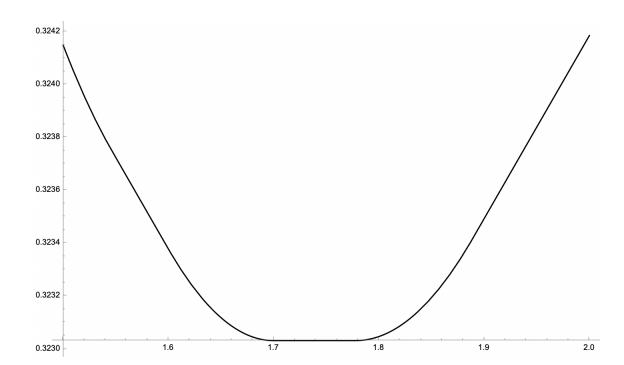
\includegraphics[width=0.58\textwidth]{assets/fig/_page_187_Figure_2.jpeg}
  \caption{\(\xi \in [1.5, 2]\) 范围内 \((2/17^2)(9\xi + I_{\xi}^{17}(\xi))\) 的函数图像片段，显示区间 \(\xi \in [1.7, 1.78]\) 被包含在极小值化范围内.}\label{fig:14.5.1}
\end{figure}

对于分母速率, 先前的计算此时修改为:
\begin{equation}\label{eq:14.5.3}
\tau^{\flat}(\mathbf{b}) = \frac{1 \cdot 0 + (3+5) \cdot 2 + (7+9+11+13+\ldots+33) \cdot 4}{17^2} = \frac{1136}{289},
\end{equation}
并且, 由图~\ref{fig:14.5.1}（其揭示了 \(\xi \in [1.7, 1.78]\) 被包含在极小值化区间内）:

\begin{equation}\label{eq:14.5.4}
\begin{aligned}
\tau^{\sharp}(\mathbf{e}) &= \frac{2}{m^{2}} \min_{\xi \in [0, m]} \left\{ \xi \sum_{i=1}^{m} e_{i} \right. \\
&\quad + \left. \left( \max_{1 \leq i \leq m} e_{i} \right) I_{\xi}^{m}(\xi) \right\} \\
&= \min_{\xi \in [0, 17]} \left\{ (2/17^{2}) \left( 9\xi + I_{\xi}^{17}(\xi) \right) \right\} \\
&= (2/17^{2}) \left( 9 \cdot 7/4 + I_{7/4}^{17}(7/4) \right) = \frac{78419}{242760}.
\end{aligned}
\end{equation}
因此, 我们此时获得了:
\begin{equation}\label{eq:14.5.5}
\tau(\mathbf{b}; \mathbf{e}) = \tau^{\flat}(\mathbf{b}) + \tau^{\sharp}(\mathbf{e}) = \frac{1136}{289} + \frac{78419}{242760} = \frac{1032659}{242760} = 4.2538...,
\end{equation}
这正是在等式 (A.6.2) 中浮现的数值 \(\frac{1032659}{242760}\).

\begin{proof}
我们现在可以通过推导 m < 17 形式的矛盾来再次完成证明. 
以及类似于定理 A 的证明, 这可以通过若干种方式来进行. 
例如：应用定理 7.0.1, 我们获得了公式 (A.6.2) 中计算出的上界 \(m \le 16.2\).
\end{proof}